\providecommand{\main}{..}
\documentclass[\main/master.tex]{subfiles}
\begin{document}
\chapter{Presentation}\label{chp:example-1}




\subsection{Cavendish Experiment}
Torsion Pendulum is an oscillator made of mass hung by a string from a fixed point so it could swing free. The Cavendish experiment, first performed in the 17th century, measures the gravitational force between masses using a torsional pendulum.
\par 
Assuming no friction or other damping force (simple harmonic oscillator) when a mass is interduced, there are two sources of torque in the system; restoring tourqe by wire torsion and by gravitational force. At equilibrium, tourqes are canceled out at an angle $\theta$.

\begin{figure}[htbp]
	\centering
	\fbox{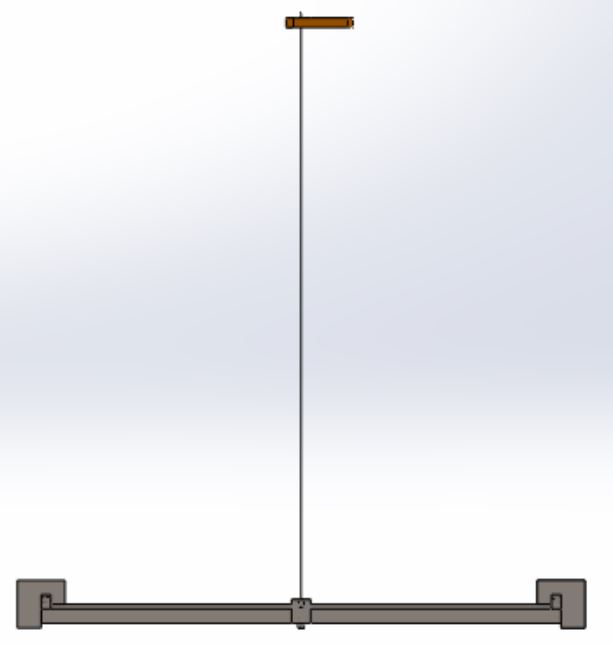
\includegraphics[scale=1.2]{\main/images/2 - theoretical background/torsion_pendulum.JPG}}
	\caption[pendulum]{a torsion pendulum}
	\label{fig:torsion_pendulum}
\end{figure}
\begin{equation}
\overrightarrow{\tau} = \kappa\theta = LF = L\frac{GmM}{r^2}    \label{eqn:gravitation_tourqe}
\end{equation}

\subsection{System Noises}
\subsection{System Design}
The pendulum is placed inside vacuum chamber to reduce noises, with a front mirror to measure angle displacement. The chamber build is  with two small viewports on the sides, used by the PID system to damp noises, one in front of the pendulum's mirror. 
\par
Measurement is made when valve closed and engine off, to prevent rotation noise.






\end{document}